The use of laser interferometers allows for the detection of gravitational waves at sites such as LIGO~\cite{Abbott_2009, Aasi_2015}, Virgo~\cite{Acernese_2008, Acernese_2014} and KAGRA~\cite{10.1093/ptep/ptx180}. These form the current second generation of GW observatories, which have opened the field of gravitational wave (GW) astronomy. The second-generation detectors are, however, approaching their design sensitivities, with future upgrades reaching the facility limits. As many science cases require an improvement in sensitivity by roughly one order of magnitude, a new third generation of detectors is being proposed. One of these is the Einstein Telescope (ET) \cite{Punturo_2010, Hild_2011}, which will be based in Europe. 
This chapter introduces ET, outlining the detection principle, its conceptual design and scientific goals.

\section{Interferometric Detection}

%  TODO: citation, also better figure maybe
\begin{figure}
	\centering
	\makebox[\textwidth]{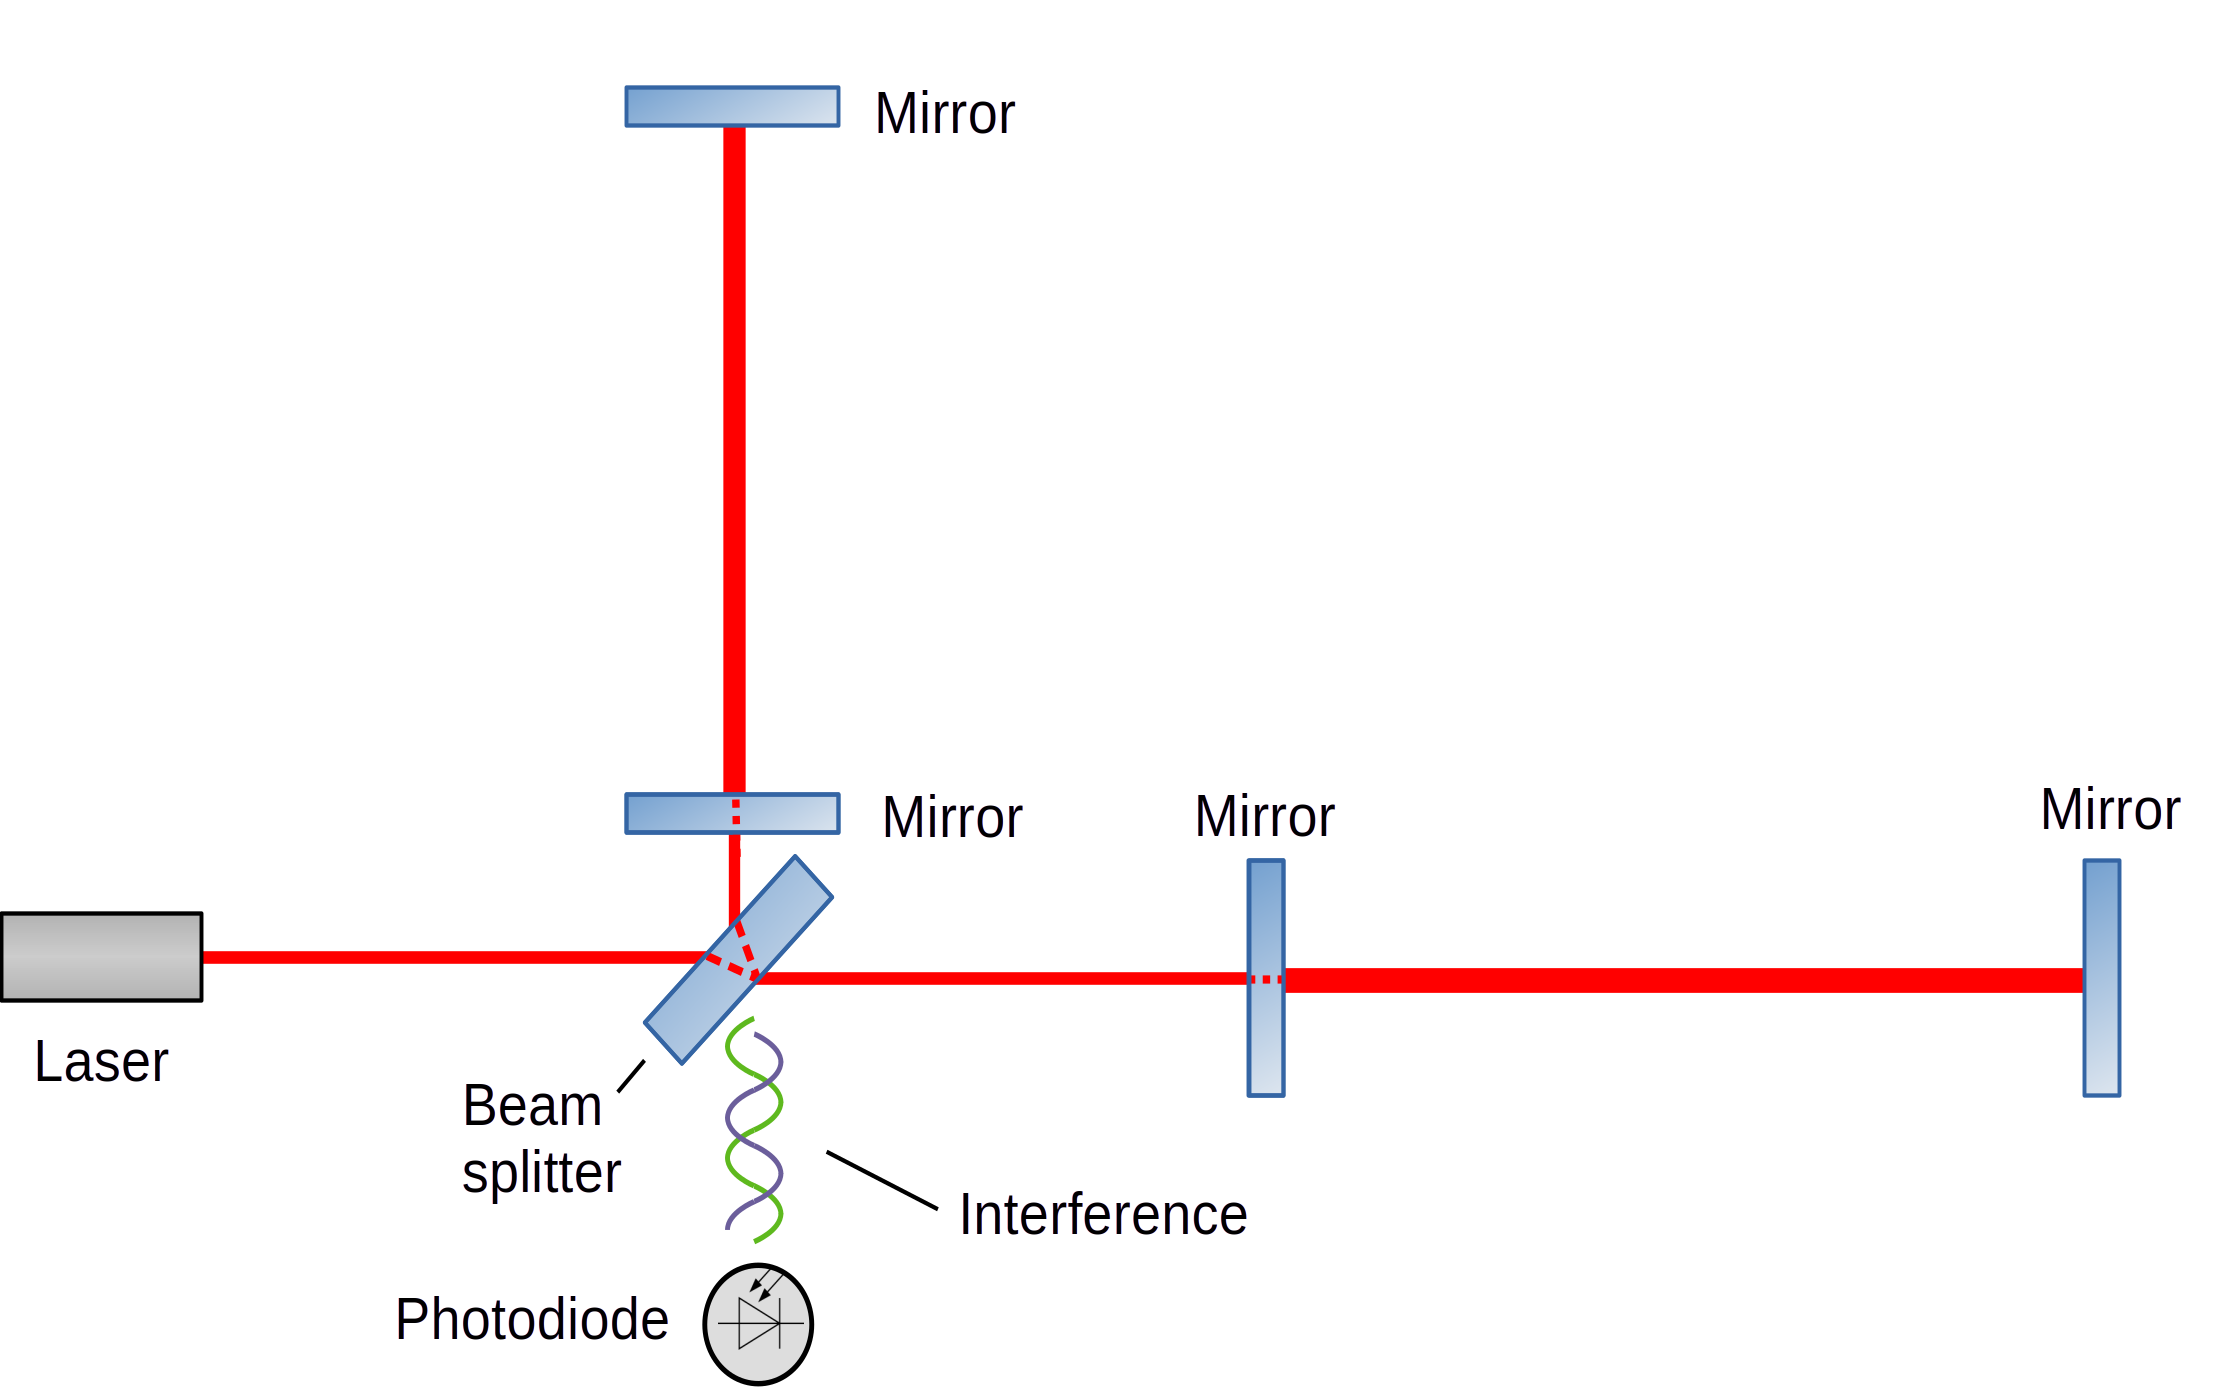
\includegraphics[width=14cm]{the_einstein_telescope/images/michelson/michelson}}
	\caption{Michelson laser-interferometer schematic, not drawn to scale. Usually, both arms will be of equal length. The extra mirrors near the beam splitter form power-enhancing \emph{Fabry-Perot cavities}.}
	\label{fig:einstein_telescope:michelson}
\end{figure}	

Ch.~\ref{sec:gravitational_waves:production} showed that the GW perturbations as measured on Earth are incredibly tiny, with amplitudes of $h \lesssim \SI{E-21}{}$, posing a significant challenge for direct detection. GWs are measured directly by observing their effect on test masses. From Eqs.~\ref{eq:gravitational_waves:plus_polarization} and \ref{eq:gravitational_waves:cross_polarization}, it is clear that a passing GW will cause displacement of the same order of magnitude as the perturbation $h$. This effect can be exploited using a \emph{Michelson laser interferometer} with its mirrors serving as the test masses. 

In the simplest case, this instrument consists of one laser, a beam splitter, two mirrors and a photo diode. The laser is directed towards the partially reflective beam splitter. The photons are sent down the two interferometer arms and reflected by mirrors at each end. The two beams travel back to the beam splitter where they are redirected to the photodiode measuring the resulting interference. 
A schematic is shown in Fig.~\ref{fig:einstein_telescope:michelson}.
The instrument is calibrated such that, in the absence of a GW, the beams interfere destructively at the photodiode. This is called \emph{dark fringe operation}.

This setup is enhanced by the inclusion of extra mirrors forming so-called \emph{Fabry-Perot cavities} with those mirrors at the end of each arm (see Fig.~\ref{fig:einstein_telescope:michelson}). The cavities increase the effective arm length as photons bounce back and forth a few hundred times before reaching the beam splitter again.

Now, suppose a purely plus polarized GW passes along the z-direction, 
and interferometer's arms lie on the x-axis and the y-axis. If the arms are of length $L$, the GW will cause length changes of  
$\Delta L_x = h_+L/2$ and $\Delta L_y = -h_+L/2$
respectively (see Eq.~\ref{eq:gravitational_waves:plus_polarization}). This leads to a path difference 
\begin{equation}
	\label{eq:einstein_telescope:path_difference}
	\Delta L = \Delta L_x - \Delta L_y = h_+L,	
\end{equation} 
which results in a phase difference of $\Delta \phi = (2\pi/\lambda) \Delta L$ with the laser wavelength $\lambda$. For arms of $\pazocal{O}(\SI{1}{\kilo\meter})$ the path differences will be $\pazocal{O}(\SI{E-18}{\meter})$, which is much smaller than typical laser wavelengths of $\pazocal{O}(\SI{E-6}{\meter})$. Thus, phase difference produces a small deviation from destructive interference and the measured photodiode voltage will be proportional to the path difference. 
After calibrating the detector, the photodiode output can be converted to path differences, which, according to Eq.~\ref{eq:einstein_telescope:path_difference}, can be divided by the arm length to yield the perturbation $h_+$. 

In fact, Eq.~\ref{eq:einstein_telescope:path_difference} can be generalized for GWs of any polarization and any propagation direction. The path length change divided by arm length will then be
\begin{equation}
	\label{eq:einstein_telescope:strain}
	\frac{\Delta L}{L} = F_+h_+ + F_\times h_\times,
\end{equation}
where $F_+$ and $F_\times$ are in $\pazocal{O}(1)$. This quantity is called the \emph{strain}, which is the projection of the GW onto the detector, and serves as the data which is used for further analysis. In an act of notation abuse, the GW strain is denoted $h$, not to be confused with the trace of $h_{\mu\nu}$. $F_+$ and $F_\times$ are the \emph{antenna pattern functions}. For a GW with polarization $\psi$ and incoming direction given by $\theta$ and $\varphi$, the polar and azimuth angles, these read
\begin{align}
	\label{eq:einstein_telescope:antenna_functions}
	\begin{split}
		F_+ = \frac{\sin\gamma}{2}((1+\cos^2\theta)\cos2\varphi\cos2\psi - 2\cos\theta\sin2\varphi\sin2\psi), \\
		F_\times = \frac{\sin\gamma}{2}((1+\cos^2\theta)\cos2\varphi\sin2\psi + 2\cos\theta\sin2\varphi\cos2\psi).
	\end{split}
\end{align}
Here, the interferometer arm lies on the x--y plane with one arm on the x-axis while the other one is rotated by $\gamma$, which denotes the detector opening angle. Notice that there are four cases where both pattern functions vanish. These are the blind spots of the detector, which occur for GWs that propagate along the detector plane, \emph{i.e.}\ $\theta=\pi/2$. Then the interferometer is blind to those GWs with incident azimuth angles $\varphi$ of \SI{45}{\degree}, \SI{135}{\degree}, \SI{225}{\degree} and \SI{315}{\degree}.

\begin{figure}
	\centering
	\makebox[\textwidth]{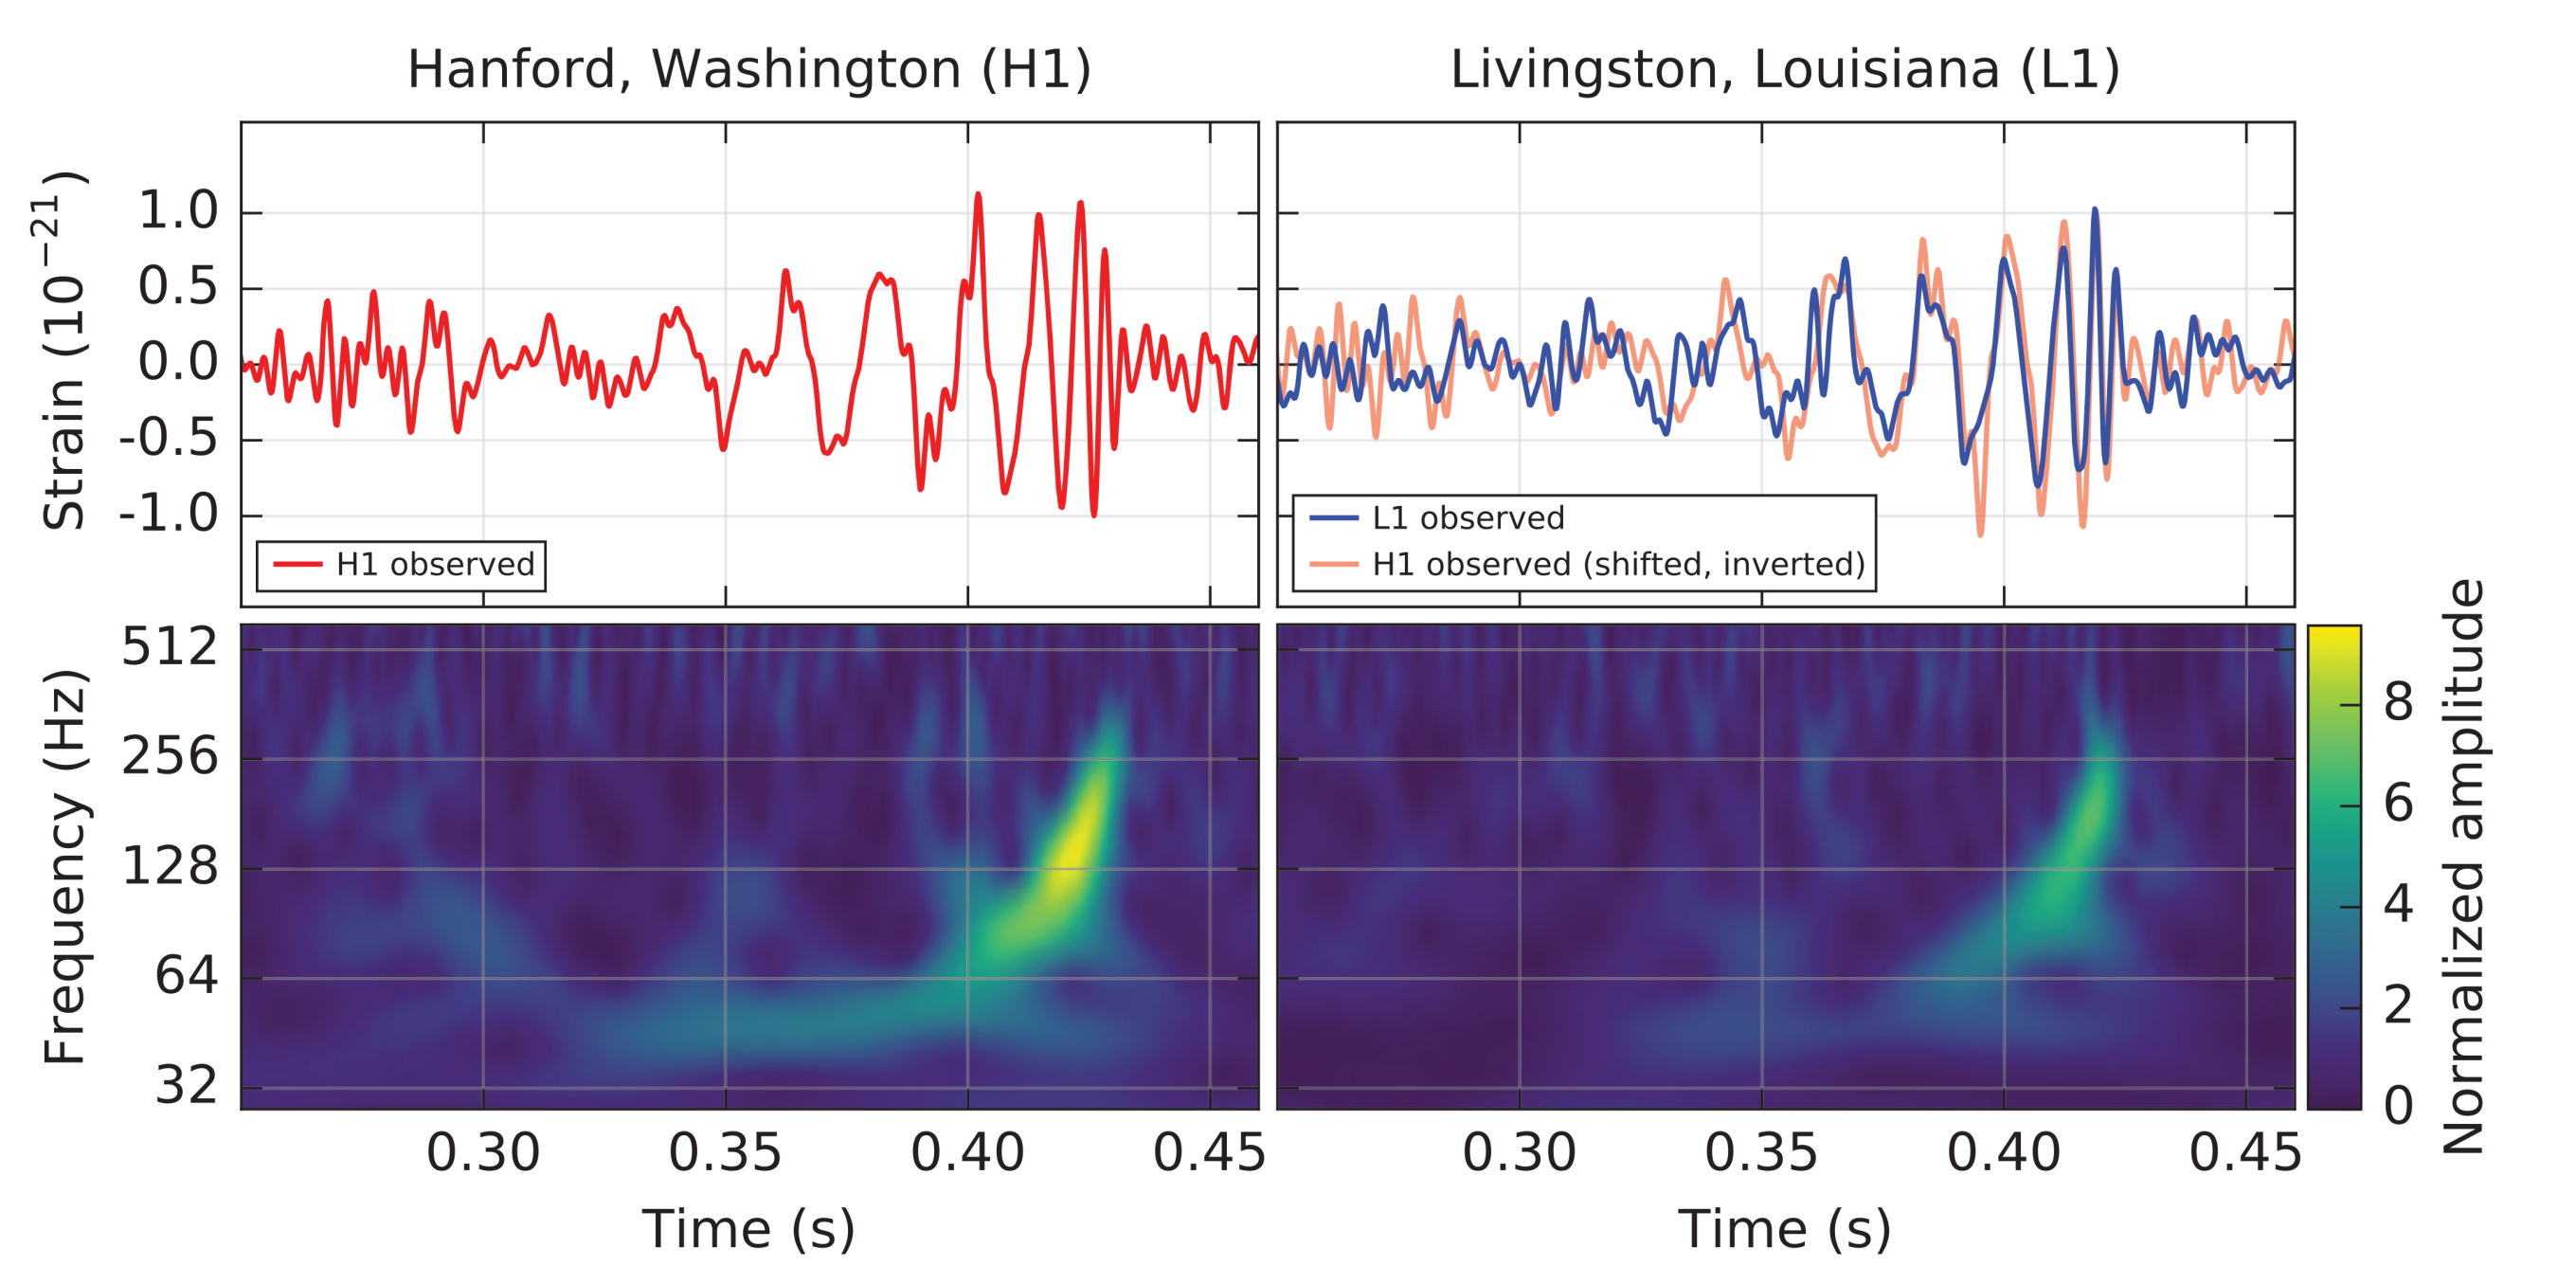
\includegraphics[width=16cm]{the_einstein_telescope/images/gw150914_plot_cropped}}
	\caption{GW150914 as measured at the two LIGO sites, H1 (\emph{left column}) and L1 (\emph{right column}) shifted by \SI{7}{\milli\second} and inverted to make up for the detectors' relative position and orientation. Strain (\emph{top row}) and spectogram (\emph{bottom row}). The data is bandpassed from \SI{35}{\hertz} to \SI{350}{\hertz} for visualization. Adapted from \cite{PhysRevLett.116.061102}.}
	\label{fig:einstein_telescope:gw150914}
\end{figure}	

\begin{figure}
	\centering
	\makebox[\textwidth]{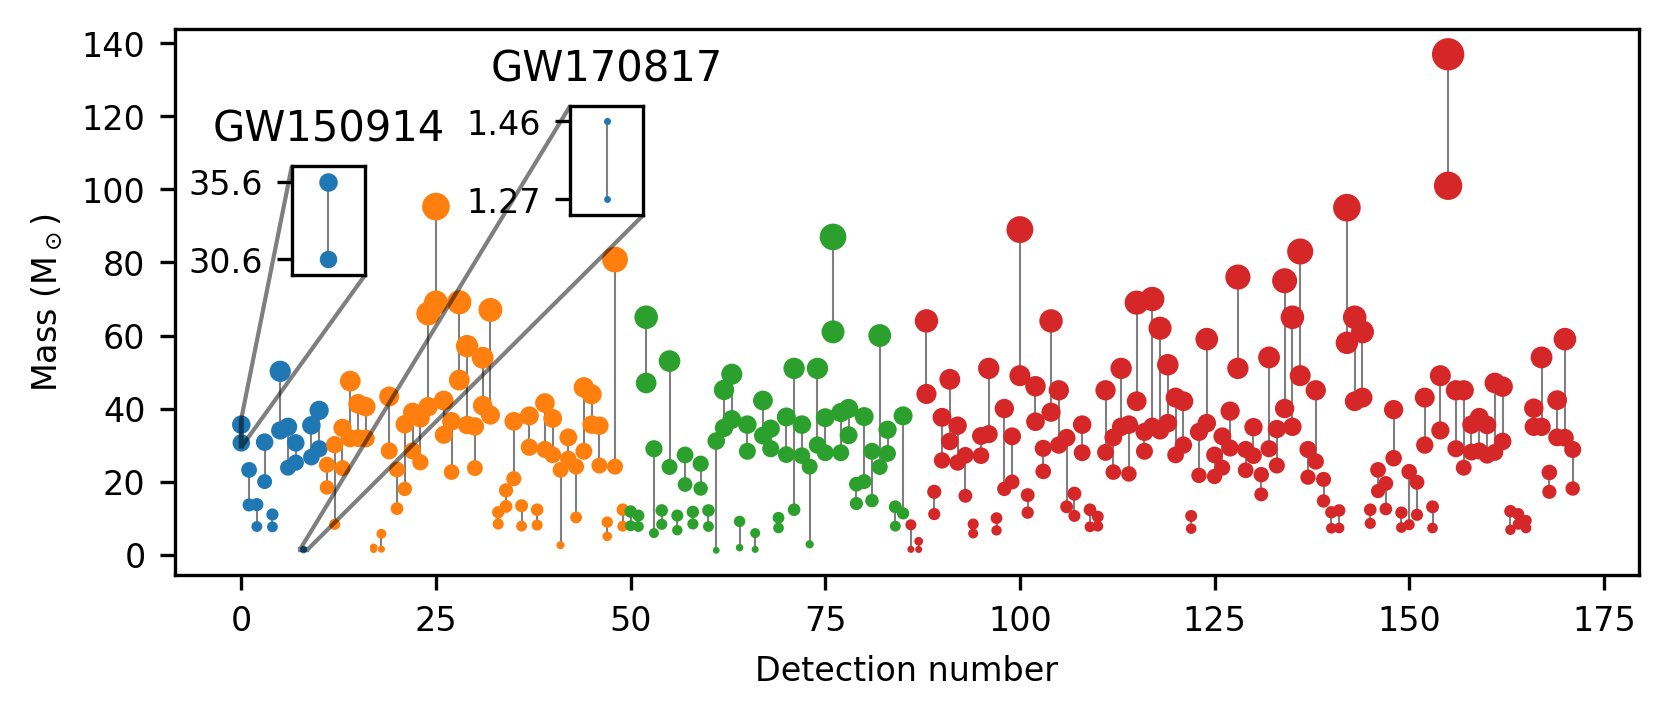
\includegraphics[width=15cm]{theory_of_gravitational_waves/images/population/population}}
	\caption{CBCs observed by LIGO, Virgo and KAGRA in their four observing runs, each plotted in a different color. Each merger is represented as two dots denoting the two component masses (in both y-value and dot size). Data from \cite{PhysRevX.9.031040, PhysRevX.11.021053, PhysRevX.13.041039, theligoscientificcollaboration2025gwtc40updatinggravitationalwavetransient}, uncertainties are not plotted.}
	\label{fig:einstein_telescope:population}
\end{figure}

This detection principle is employed with great success at LIGO, which consists of two interferometers, H1 and L1, separated by \SI{3000}{\kilo\meter}. These have arm lengths of \SI{4}{\kilo\meter} and \SI{90}{\degree} opening angles. The two sites allow for the rejection of false signals via coincident detection ($<\SI{10}{\milli\second}$, the time-of-flight between the two detectors). LIGO achieved the first direct detection of a GW signal on September 14th, 2015 \cite{PhysRevLett.116.061102} resulting in a Nobel prize award in 2017 \cite{nobel2017}. The signal was identified as a BBH merger with masses $36^{+5}_{-4}\,\SI{}{\solarmass}$ and $29^{+4}_{-4}\,\SI{}{\solarmass}$ and with a luminosity distance of $410^{+160}_{-180}\,\SI{}{\mega\parsec}$. GW signals are conventionally labeled based on their arrival time, so GW150914 in this case. See the measured signal in Fig.~\ref{fig:einstein_telescope:gw150914}. So far, the LIGO, Virgo and KAGRA observatories have made more than 200 confident GW detections in the span of four observing runs \cite{PhysRevX.9.031040, PhysRevX.11.021053, PhysRevX.13.041039, theligoscientificcollaboration2025gwtc40updatinggravitationalwavetransient}. The majority of these are black hole mergers. BNS mergers are identified based on the component masses which have to be $\lesssim\SI{2}{\solarmass}$. The first direct detection of a neutron star merger was GW170817 \cite{Abbott_2017}. See the signals for which component masses are provided in Fig.~\ref{fig:einstein_telescope:population}.

%\begin{figure}
%	\centering
%	\makebox[\textwidth]{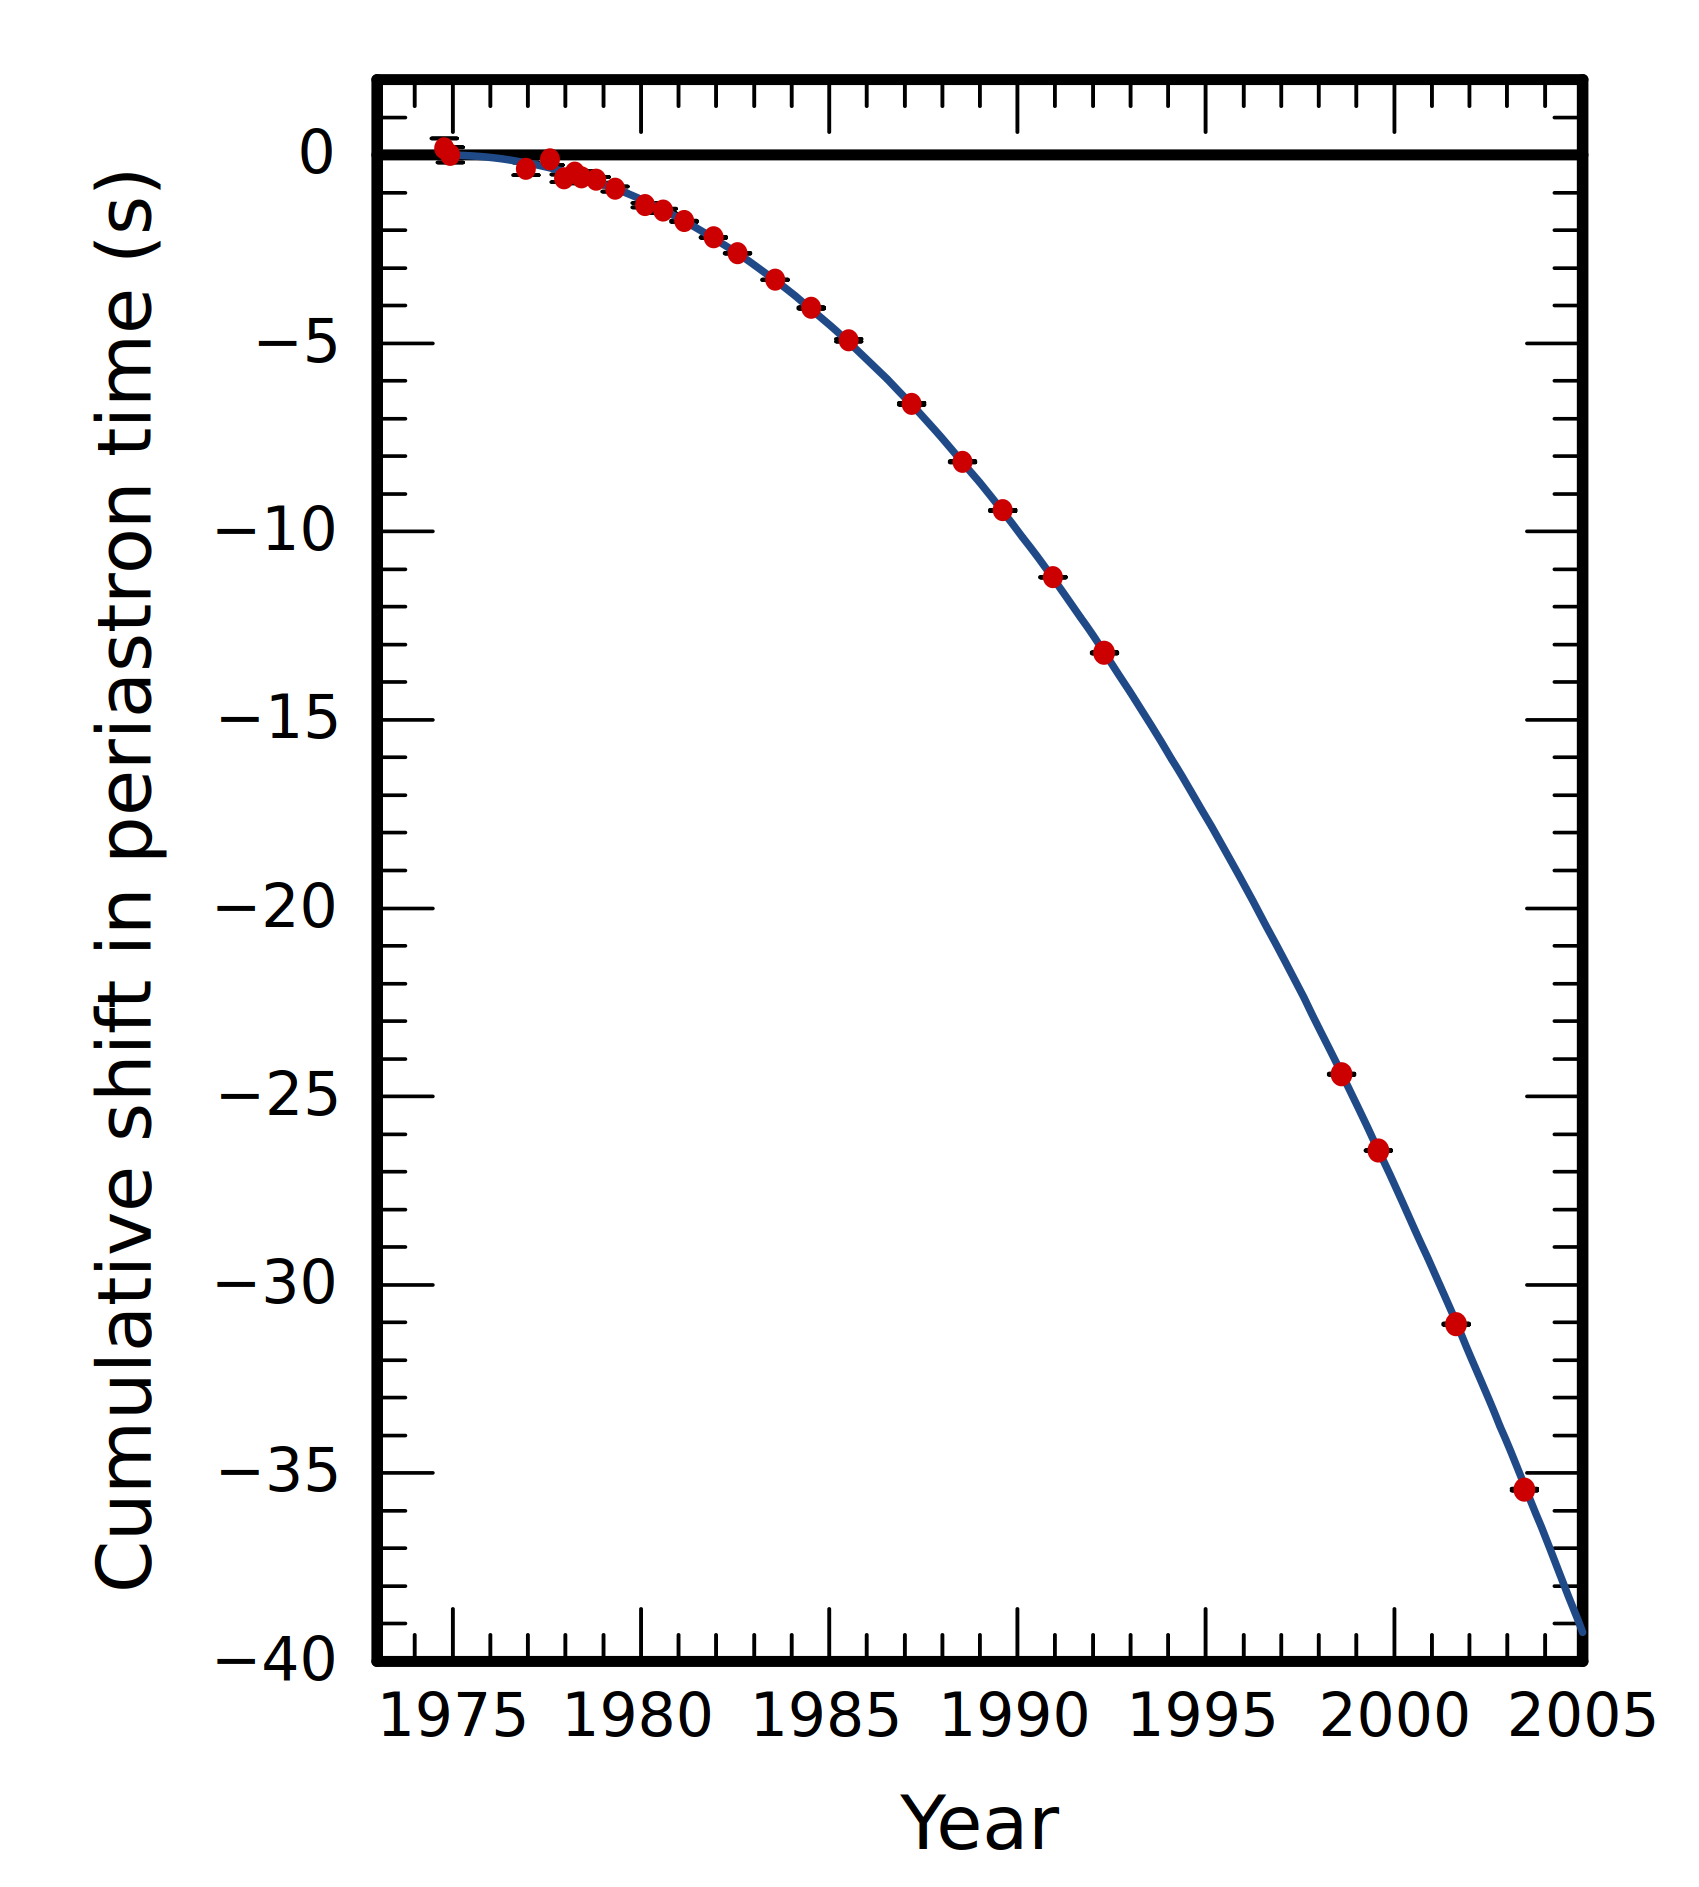
\includegraphics[width=8cm]{the_einstein_telescope/images/hulse_taylor_wiki}}
%	\caption{}
%	\label{fig:einstein_telescope:hulse_taylor}
%\end{figure}	

%\begin{figure}[p]
%	\centering
%	\makebox[\textwidth]{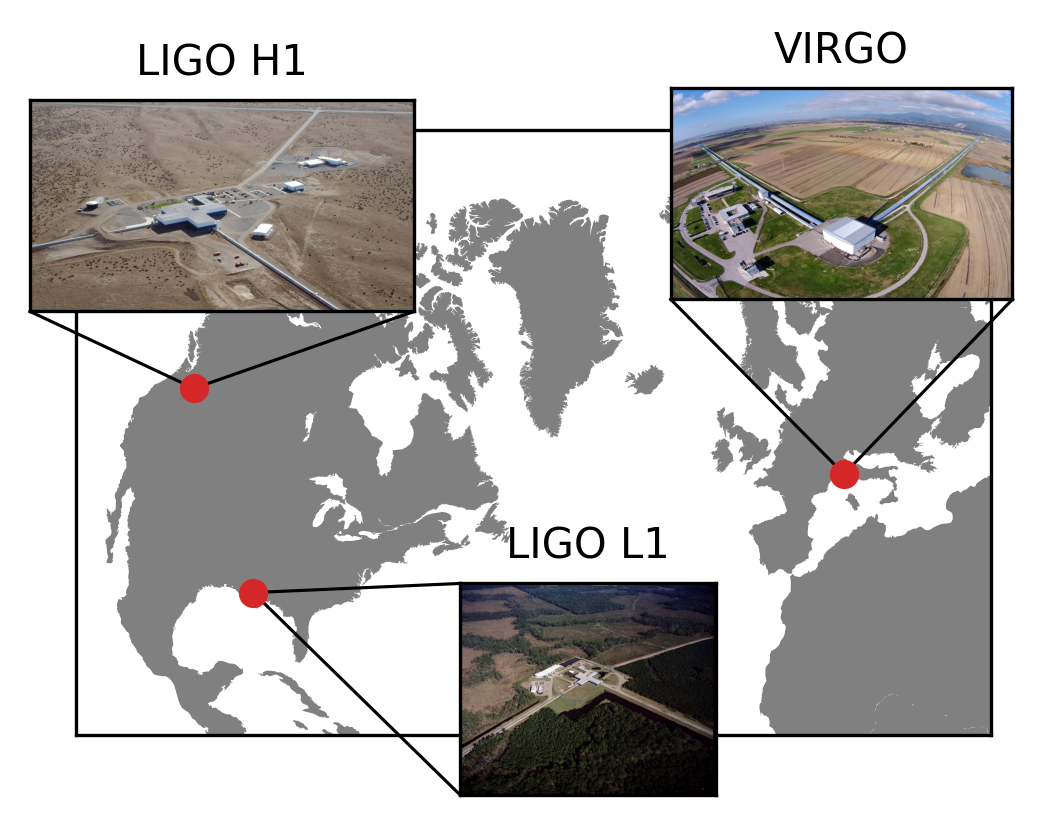
\includegraphics[width=7cm]{the_einstein_telescope/images/2nd_gen_detectors/LIGO_VIRGO}}
%	\caption{Positions of the LIGO and Virgo observatories.}
%	\label{fig:einstein_telescope:2nd_gen}
%\end{figure}	

\section{Conceptual Design}

% 10km arms
% underground -> better sensitivity
% triangle -> all sky coverage, null stream
% xylophone -> LF HF optimized
% candidates are Meuse-Rhine Euregio, or Sardinia

The Einstein Telescope (ET) aims for an increase in sensitivity of a factor ten compared to second-generation detectors, especially in the low frequency regime $\pazocal{O}(\SI{1}{\hertz})$.
To this end, the arm length will be increased to \SI{10}{\kilo\meter} yielding an overall sensitivity increase. To improve the low frequency sensitivity, where noise is mostly seismic, ET will be built \SI{200}{\meter} to \SI{300}{\meter} underground.
A detailed description of the latest ET technical design is provided by \cite{ET-0007C-20}.\footnote{It should be mentioned that this technical report is rather old as of now. In particular, it focuses solely on a triangular configuration of three nested detectors with \SI{60}{\degree} opening angles. However, the detector geometry is currently debated with 2L configurations being investigated as well (two detectors with \SI{90}{\degree} opening angles) \cite{Branchesi_2023}.}

\begin{figure}
	\centering
	\makebox[\textwidth]{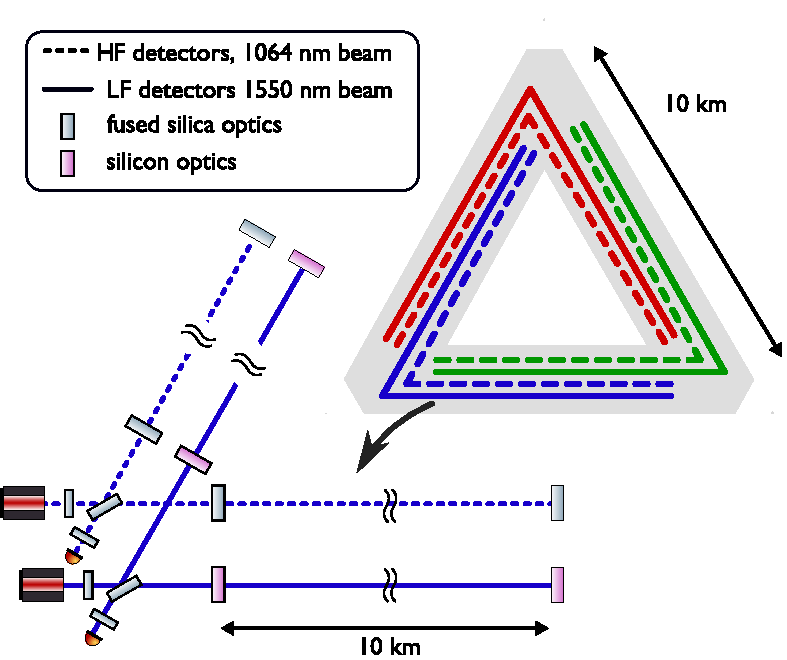
\includegraphics[width=10cm]{the_einstein_telescope/images/ET_triangle_01}}
	\caption{The ET xylophone design. Three detectors arranged in a triangular shape each consisting of a LF and HF interferometer. 
	ET-LF will feature a \SI{1550}{\nano\meter} laser wavelength and silicon optics, while ET-HF will employ a \SI{1064}{\nano\meter} laser with fused silica optics, similar to LIGO and Virgo. 
	Taken from \cite{Rowlinson_2021}.}
	\label{fig:einstein_telescope:xylphone}
\end{figure}

ET will consist of three nested detectors with \SI{60}{\degree} opening angles, arranged in a triangular pattern. 
This allows for better sky coverage at a slight sensitivity cost for interferometers with opening angles $\gamma<\SI{90}{\degree}$ (corresponding to the factor $\sin\gamma$ in Eqs.~\ref{eq:einstein_telescope:antenna_functions}). The arrangement is equally sensitive to both GW polarizations.
Each detector will comprise two interferometers, one optimized for low frequencies of \SI{3}{\hertz} to \SI{30}{\hertz} (ET-LF) and one for high frequencies \SI{30}{\hertz} to \SI{10}{\kilo\hertz} (ET-HF). This is called the \emph{xylophone} configuration. See a schematic in Fig.~\ref{fig:einstein_telescope:xylphone}. 

% noise
% quantum noise -> light power
% thermal noise -> LF: cryogenic cooling, silicon optics
% newtonian noise + seismic noise -> 

\begin{figure}
	\centering
	\makebox[\textwidth]{
		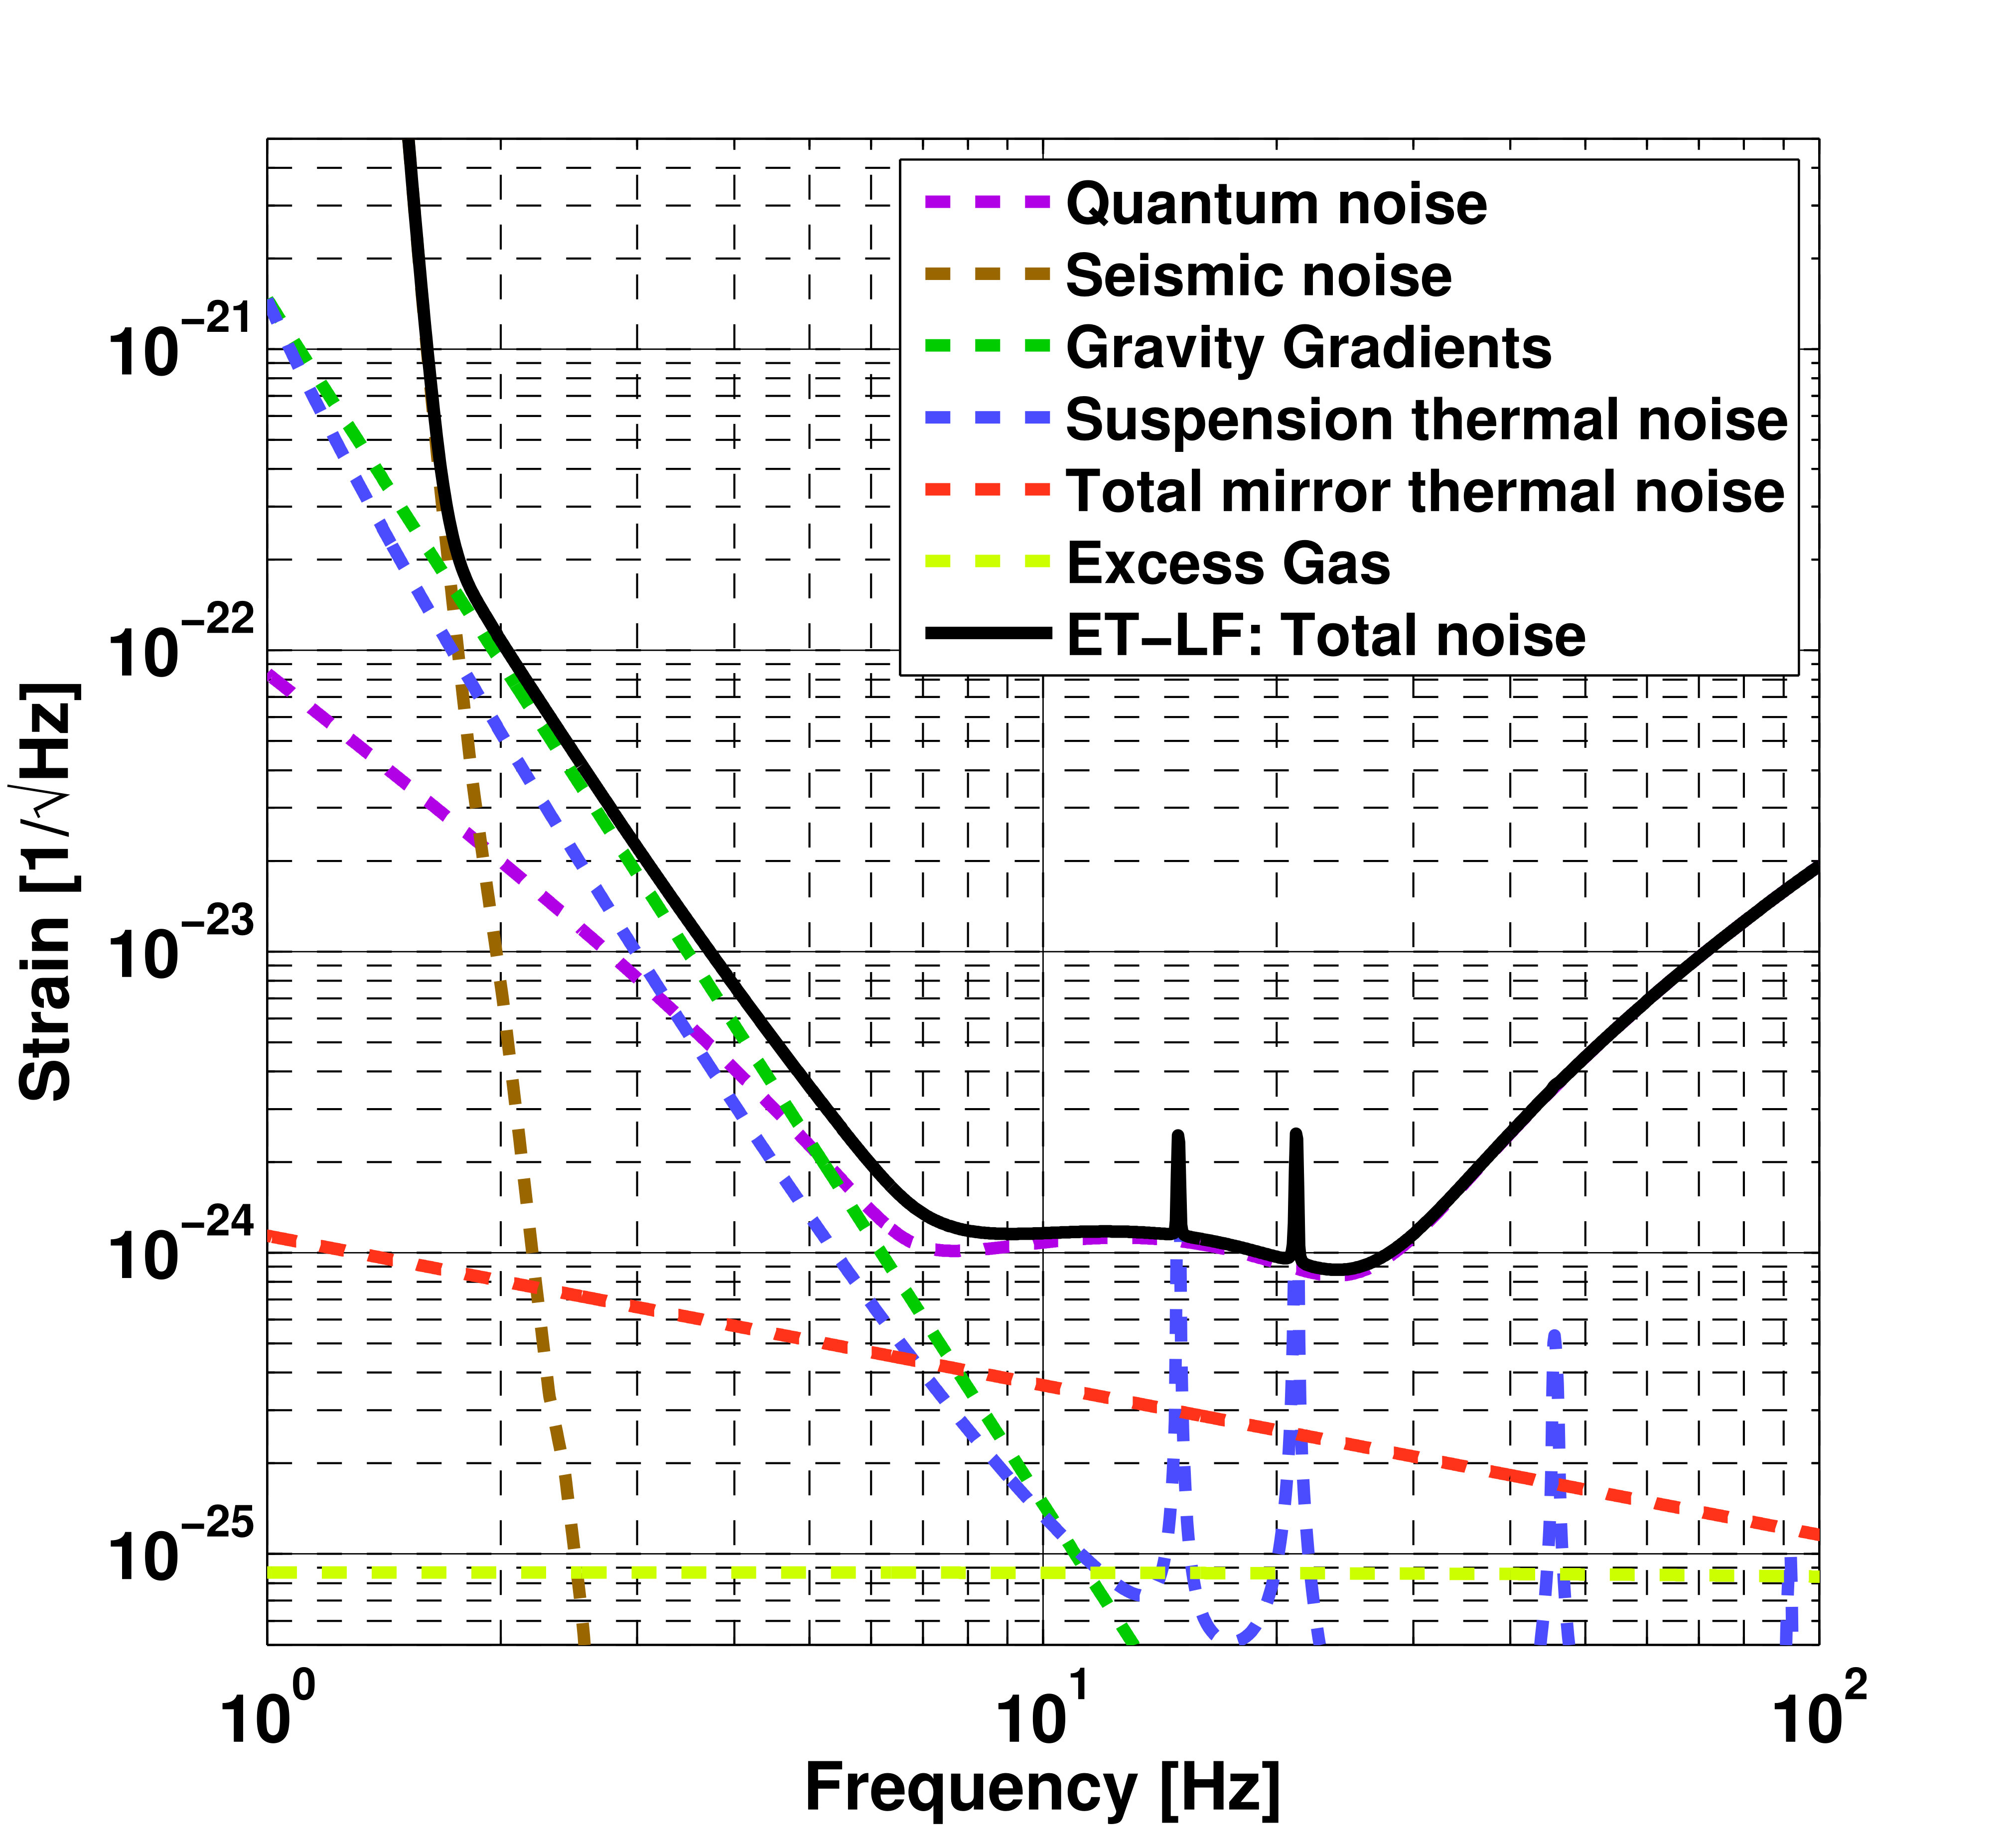
\includegraphics[width=8cm]{the_einstein_telescope/images/ETD_LF3.png}
		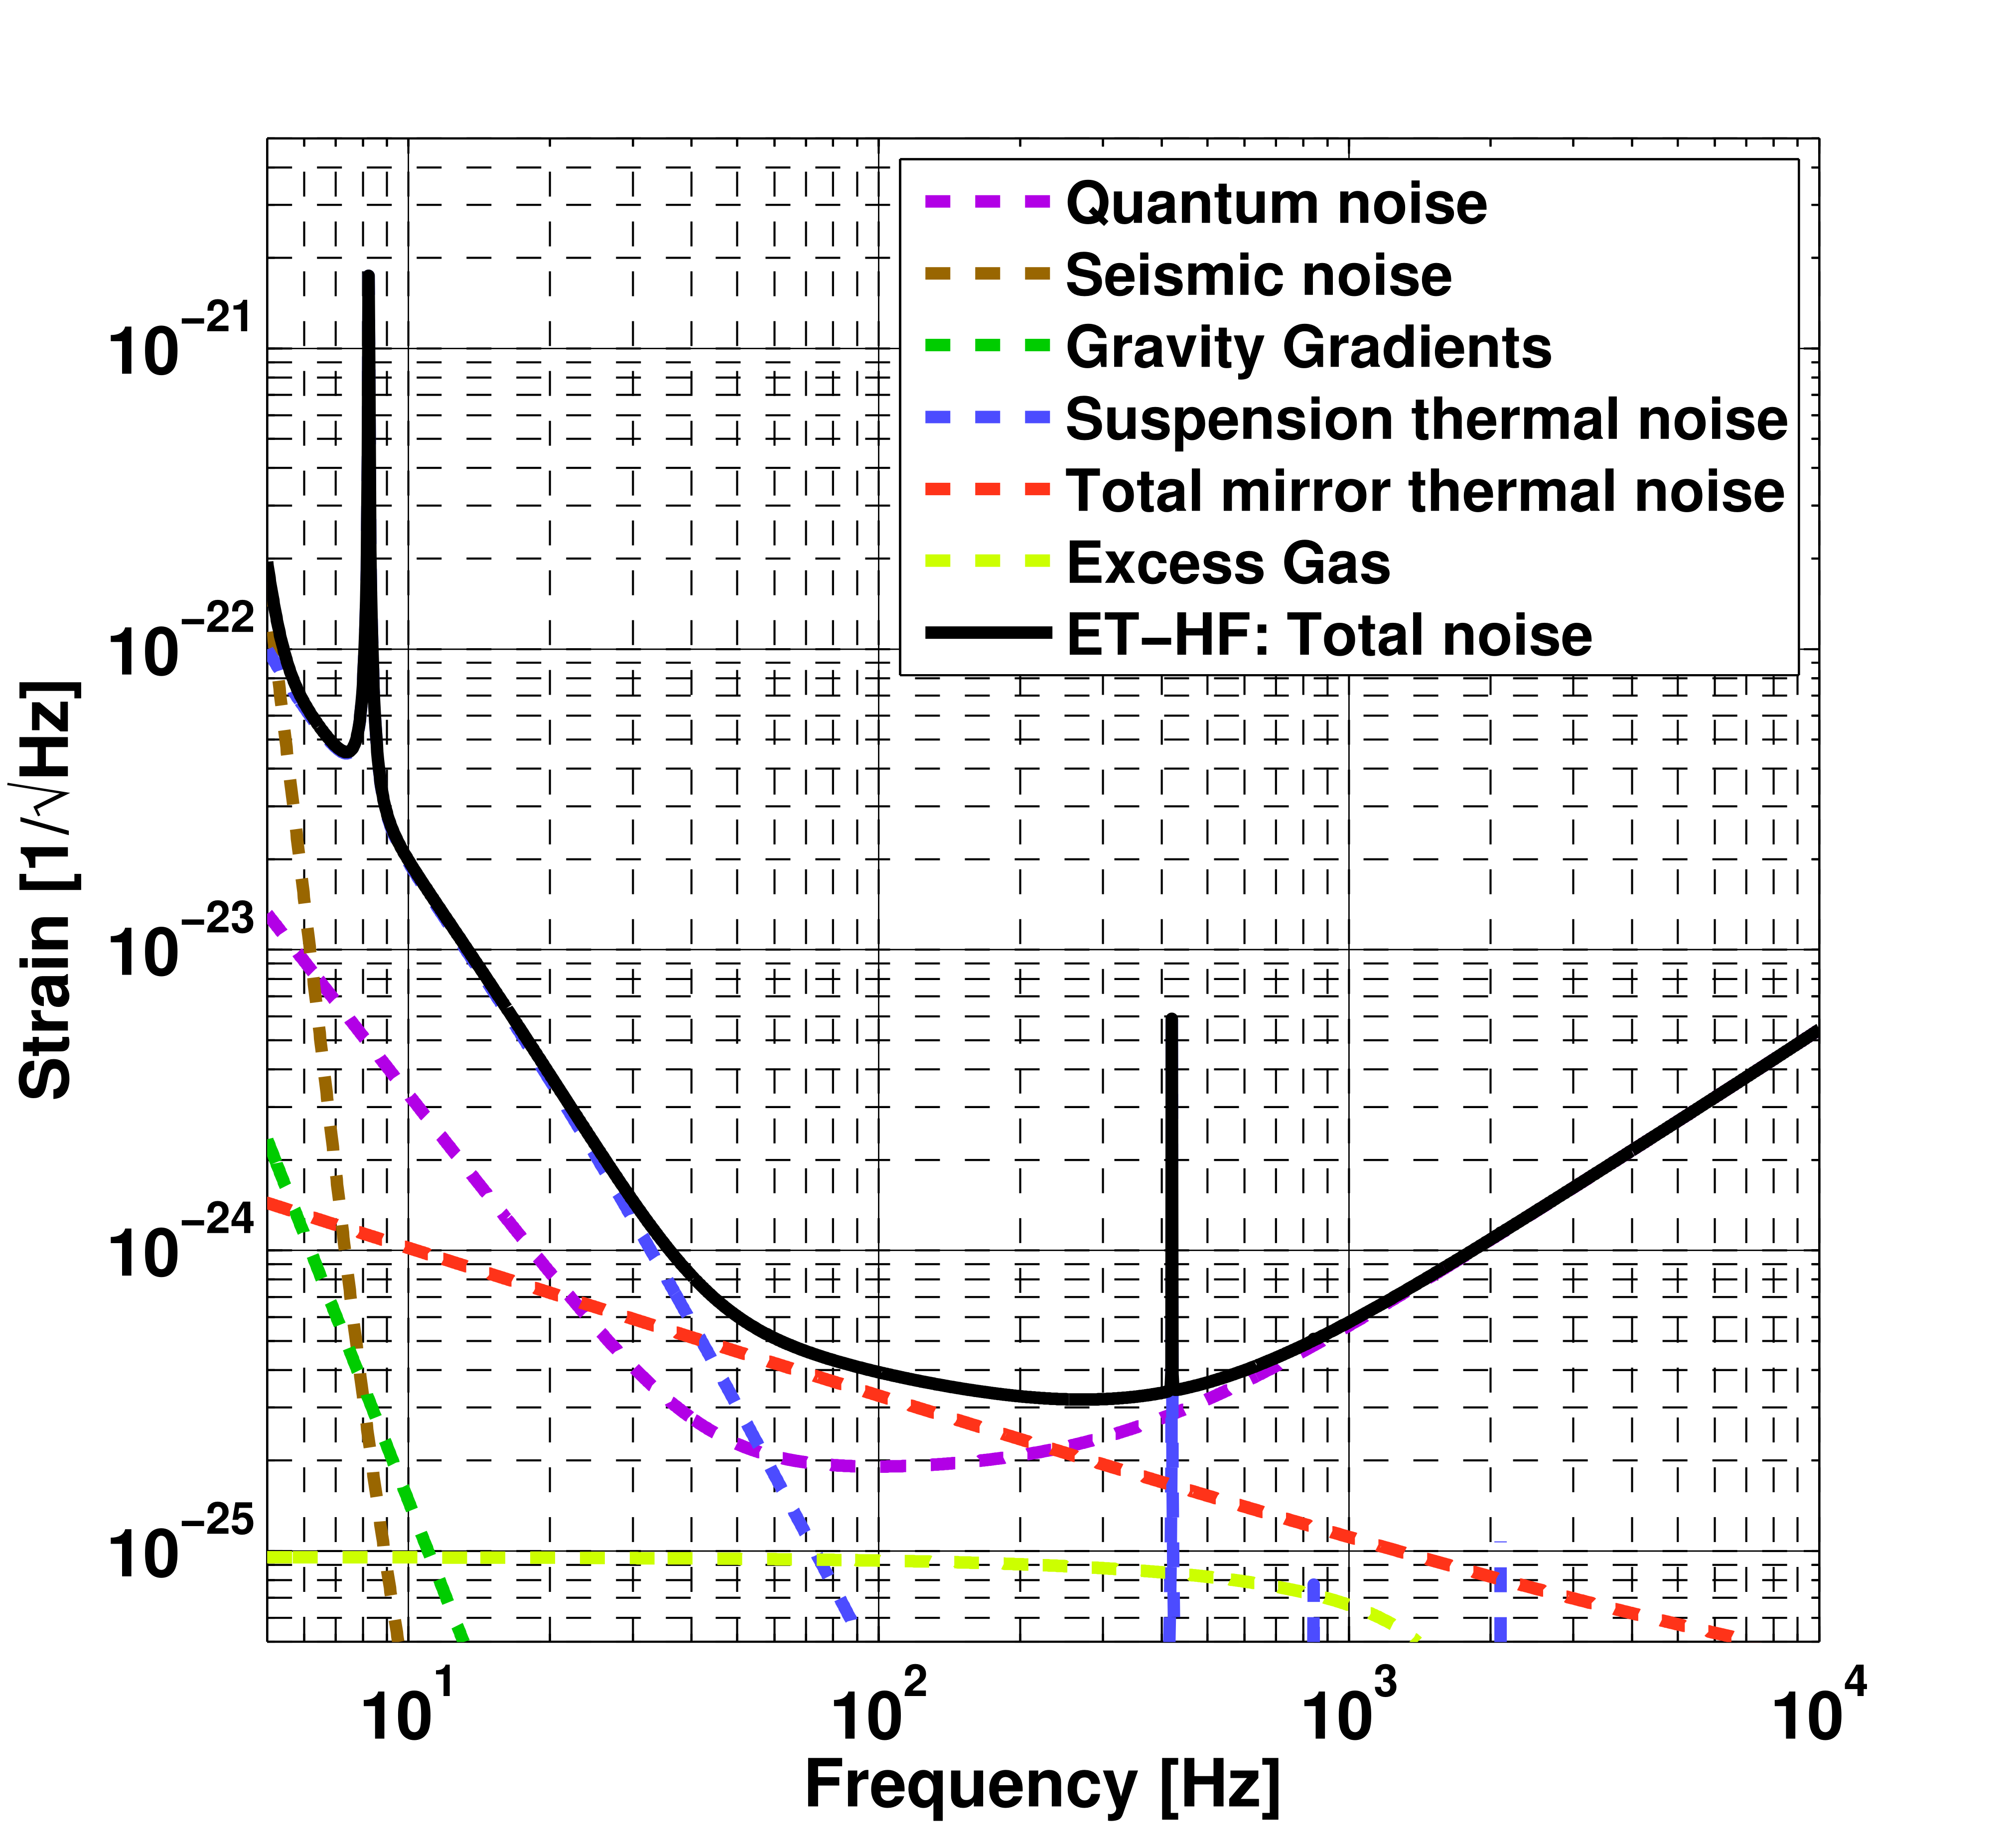
\includegraphics[width=8cm]{the_einstein_telescope/images/ETD_HF3.png}
	}
	\caption{Noise budgets for the ET-LF (left) and ET-HF (right) interferometers. The individual sources (dotted) and the total noise taken as their quadrature sum (black). The label \enquote{Gravity gradients} denotes Newtonian noise. Excess gas noise stems from residual gas in the beam tubes. Taken from \cite{Hild_2011}.}
	\label{fig:einstein_telescope:noise_budget}
\end{figure}

This configuration is useful because the main noise contribution for these instruments, the \emph{quantum noise}, behaves differently at low and high frequencies. This type of noise is caused by individual quanta of light, \emph{i.e.}\ photons, and has two components. The \emph{shot noise} results from the Poisson statistics of the total number of photons detected and dominates at high frequencies. The \emph{radiation pressure noise} arises from the momentum transfer of individual photons to the mirrors upon reflection. Fluctuations in the photon number therefore induce random displacements of the mirrors. This noise dominates at low frequencies. 

These two contributions scale oppositely with laser power: increasing the laser power reduces shot noise but increases radiation pressure.
ET-HF mitigates shot noise by operating with a higher arm cavity power of \SI{3}{\mega\watt}, while ET-LF suppresses radiation pressure by reducing the power to \SI{18}{\kilo\watt}. Compare this to the LIGO interferometers which balance both noise contributions by choosing \SI{750}{\kilo\watt}. In both ET-LF and ET-HF, radiation pressure can be further reduced by employing heavier test masses of \SI{200}{\kilo\gram} instead of \SI{40}{\kilo\gram} at LIGO.

Another noise source is \emph{thermal noise} due to Brownian motion in the test masses and their suspensions. This limits the instrument's sensitivity in the low frequencies, hence ET-LF will operate at cryogenic temperatures of \SI{10}{\kelvin} to \SI{20}{\kelvin}. The poor low-temperature behavior of fused silica, which is used for the optics of ET-HF, necessitates employing silicon for the ET-LF test masses and suspensions. Since silicon is non-transparent to wavelengths of \SI{1064}{\nano\meter}, the standard for second-generation detectors, which will be used for ET-HF as well, ET-LF will move to a larger laser wavelength of \SI{1550}{\nano\meter}.

As already mentioned, the instrument's low-frequency sensitivity is mainly limited by \emph{seismic noise} and \emph{Newtonian noise}. Both of these stem from seismic ground motion caused by local disturbances such as human activity or wind. Seismic noise describes the vibrations directly induced on the optics and can be shielded by a combination of active and passive isolation systems. ET will employ a multi-stage pendulum suspension system for its mirrors, similar to LIGO and Virgo.

Newtonian noise, on the other hand, describes disturbance of the local gravitational field caused by the mass density fluctuations associated with seismic ground motion and its effect on the test masses. Contrary to seismic noise, Newtonian noise cannot be shielded, which is the main argument for moving the detector \SI{200}{\meter} to \SI{300}{\meter} underground to a sparsely populated region. Candidates include the Euregio Meuse-Rhine and Sardinia \cite{etcandidates}.

ET is set to provide a sensitivity improvement of a factor ten, achieving a targeted sensitivity of \SI{E-24}{\hertz^{-1/2}} and broadening the frequency range down to \SI{3}{\hertz} to \SI{5}{\hertz}, compared to the current detectors' \SI{10}{\hertz} to \SI{20}{\hertz} lower limit.
See the ET noise budget for both interferometers in Fig.~\ref{fig:einstein_telescope:noise_budget}. Plotted here is the noise \emph{amplitude spectral density} (ASD) which is the square root of the \emph{power spectral density} (PSD) and is related to the root-mean-square noise amplitude at each frequency. (Ch.~\ref{sec:matched_filtering} will introduce these formally.)

\section{Scientific Goals}
 
 % -- intro paragraph --
 % black hole properties (origin (ABH, PBH -> dark matter candidate), evolution?, population)
 % neutron star properties (interior structure (QCD), population)
 % sky localization -> multi messenger (electro magnetic or neutrino follow-up from BNS)
 % new sources (CCSNe, stochastic background)
 
With its increased sensitivity, ET will detect large numbers of CBCs up to high redshifts and with unprecedented precision. In numbers that is \SI{E+5}{\nothing} to \SI{E+6}{\nothing} BBH and \SI{E+4}{\nothing} BNS signals annually \cite{abac2025scienceeinsteintelescope}. This has the potential for advances in astrophysics, cosmology and fundamental physics. For a full discussion of ET's main science cases, see \cite{ET-0007C-20, abac2025scienceeinsteintelescope}.

ET will enable the study of the stellar black hole and neutron star populations, including their mass and spin distributions, their evolution with redshift, and their formation mechanisms. ET will probe black holes beyond the epoch of star formation, possibly uncovering black holes of primordial origin. These are hypothetical non-stellar black holes, formed in the high-density conditions of the early universe, which are proposed as a dark matter candidate.

High precision measurements of CBC signatures will provide accurate tests of GR, particularly in the extreme domain during the merger phase of BBHs. Similarly, high-precision BNS signatures allow for the study of quantum chromodynamics at ultra-high density, and of possible phase transitions in the neutron star core.

ET's excellent sky coverage and sensitivity make it capable of localizing GW sources with remarkable precision. This opens the opportunity for multi-messenger astronomy, where non-GW observatories probe the source's sky location for electromagnetic or neutrino follow-ups. This is especially important for mergers involving a neutron star, which can emit both GWs and electromagnetic radiation in a kilonova \cite{Abbott_2017_kilonova}. 

Besides CBC signals, ET may detect other types of GW sources. These include signals from core collapse supernovae, continuous signals emitted by isolated rotating neutron stars, and possibly the stochastic GW background.

